
%===============================================================================
%   汎用実験レポートテンプレート（LuaLaTeX／ltjsarticle）
%===============================================================================
\documentclass[10pt,a4paper]{ltjsarticle}

%―――――― フォント設定 ―――――――
\usepackage{fontspec}            % 欧文フォント
\usepackage{luatexja-fontspec}   % 日本語フォント連携
\setmainfont{Times New Roman}    % 欧文メインフォント
\setmainjfont{IPAexMincho}       % 和文メインフォント
\setsansjfont{IPAexGothic}       % サンセリフ（見出し等）

%―――――― パッケージ群 ―――――――
\usepackage{amsmath,amssymb}     % 数式
\usepackage{graphicx,subcaption} % 画像／サブ図
\usepackage{float}               % [H] オプション
\usepackage{booktabs,multirow}   % 表組み
\usepackage[hyphens]{url}        % URL 改行
\usepackage{xurl}                % URL 柔軟改行
\usepackage{hyperref}            % ハイパーリンク
\usepackage{fancyhdr}            % ヘッダ・フッタ
\usepackage{siunitx}             % 単位

%―――――― ヘッダ・フッタ設定 ―――――――
\pagestyle{fancy}
\lhead[\bfseries\thepage]{\textbf{実験レポート}} % 左ヘッダ
\rhead[\bfseries\thepage]{作成日：\today}        % 右ヘッダ
\lfoot{学籍番号 氏名}                            % 左フッタ（要変更）
\cfoot{}                                         % 中央フッタ
\rfoot{\thepage}                                 % 右フッタ

%―――――― 各種設定 ―――――――
\graphicspath{{images/}} % 画像フォルダ
\sloppy                  % 行オーバーフロー回避

%―――――― タイトル情報 ―――――――
\title{\LARGE 実験タイトルを書く}       % レポートタイトル
\author{{\Large 学籍番号 氏名}}         % 学籍番号と氏名
\date{作成日：\today}                   % 日付

%===============================================================================
\begin{document}
%===============================================================================

\maketitle      % タイトル出力
\tableofcontents % 目次
\newpage         % 改ページ

%===============================================================================

% ここから本文
\section{基本課題}

\subsection{1--1}
R3のB1Fから4Fまでの直近２日のCO2濃度推移を以下に示す。

\begin{figure}[H]
  \centering
  \begin{subfigure}[b]{0.45\columnwidth}
    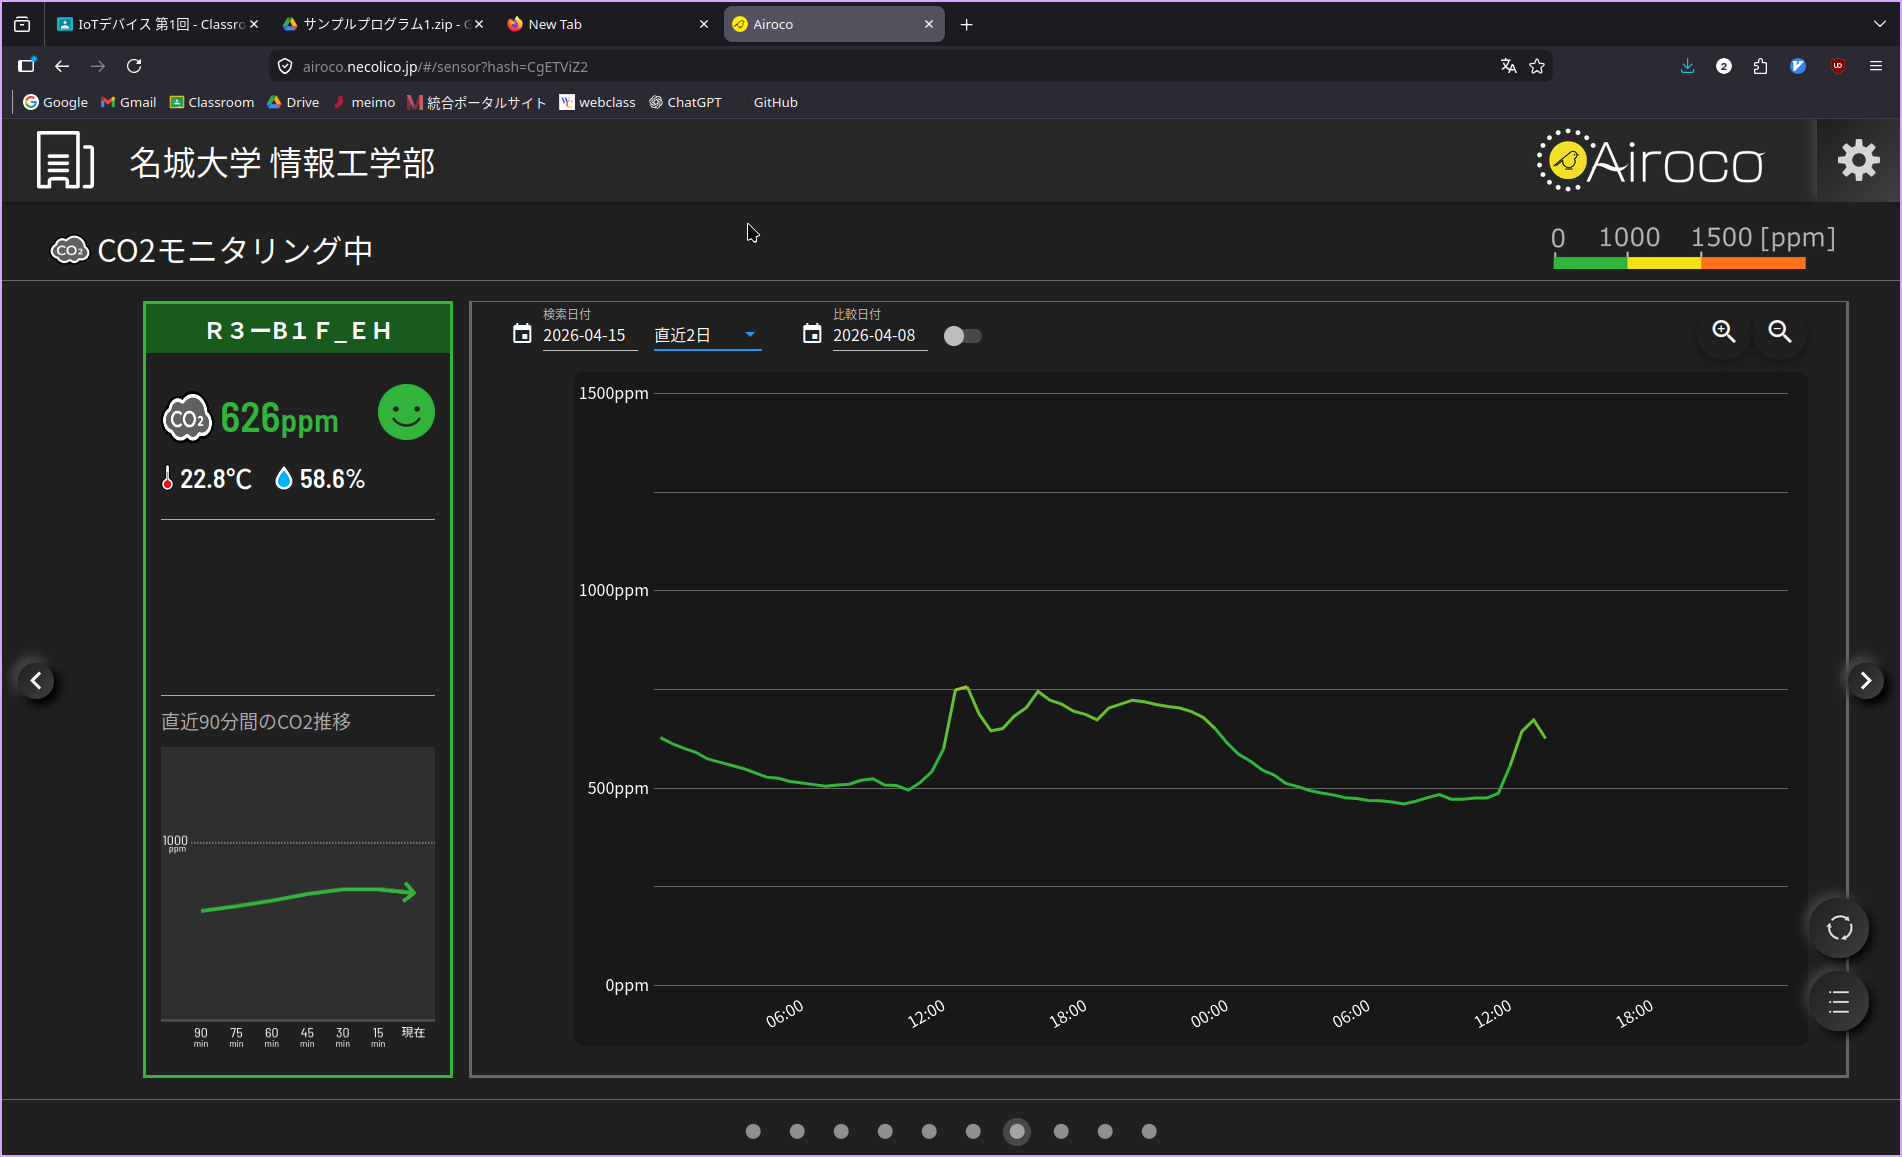
\includegraphics[width=\linewidth]{R3-B1F_EH.png}
    \caption{B1FエレベーターホールのCO2濃度}\label{fig:B1F}
  \end{subfigure}\hfill
  \begin{subfigure}[b]{0.45\columnwidth}
    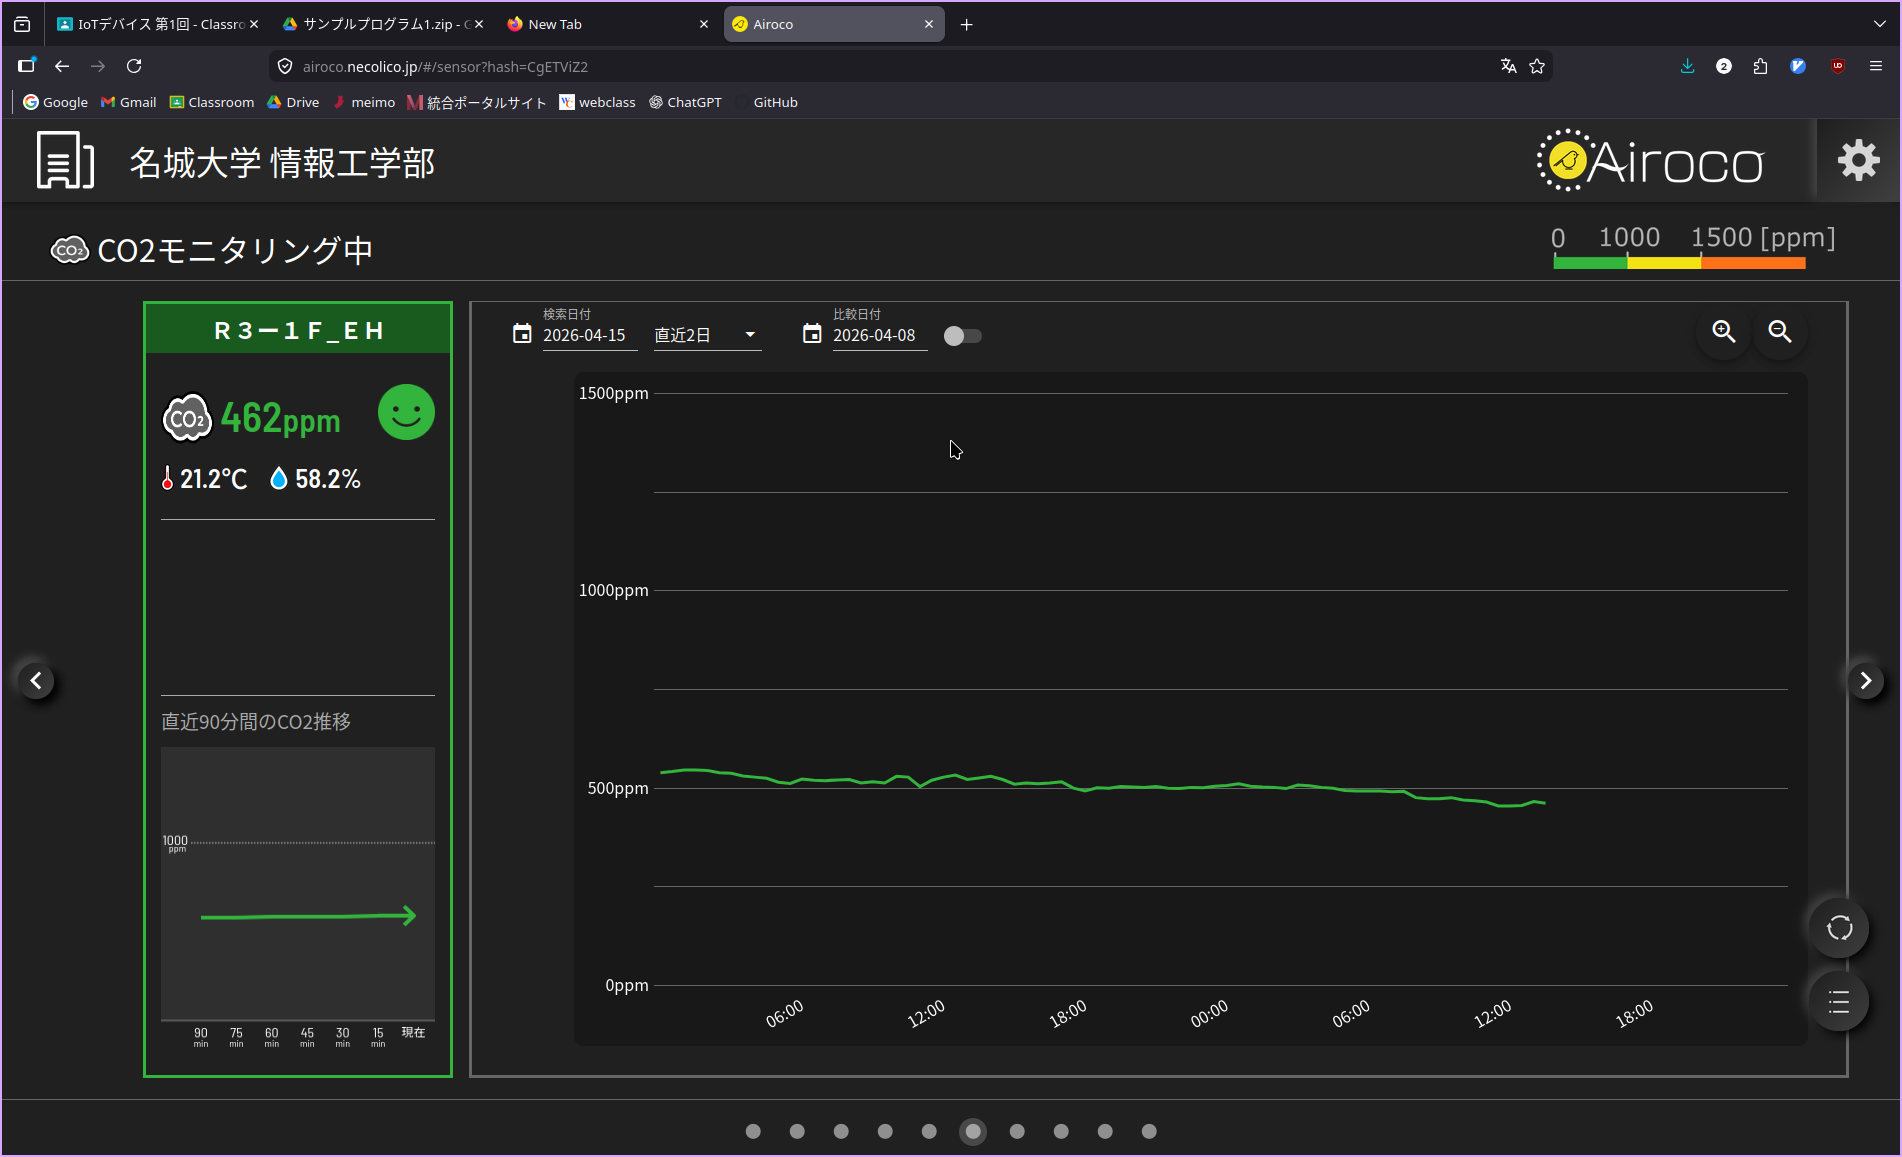
\includegraphics[width=\linewidth]{R3-1F_EH.png}
    \caption{1FエレベーターホールのCO2濃度}\label{fig:1F}
  \end{subfigure}

  \vspace{1em}

  \begin{subfigure}[b]{0.45\columnwidth}
    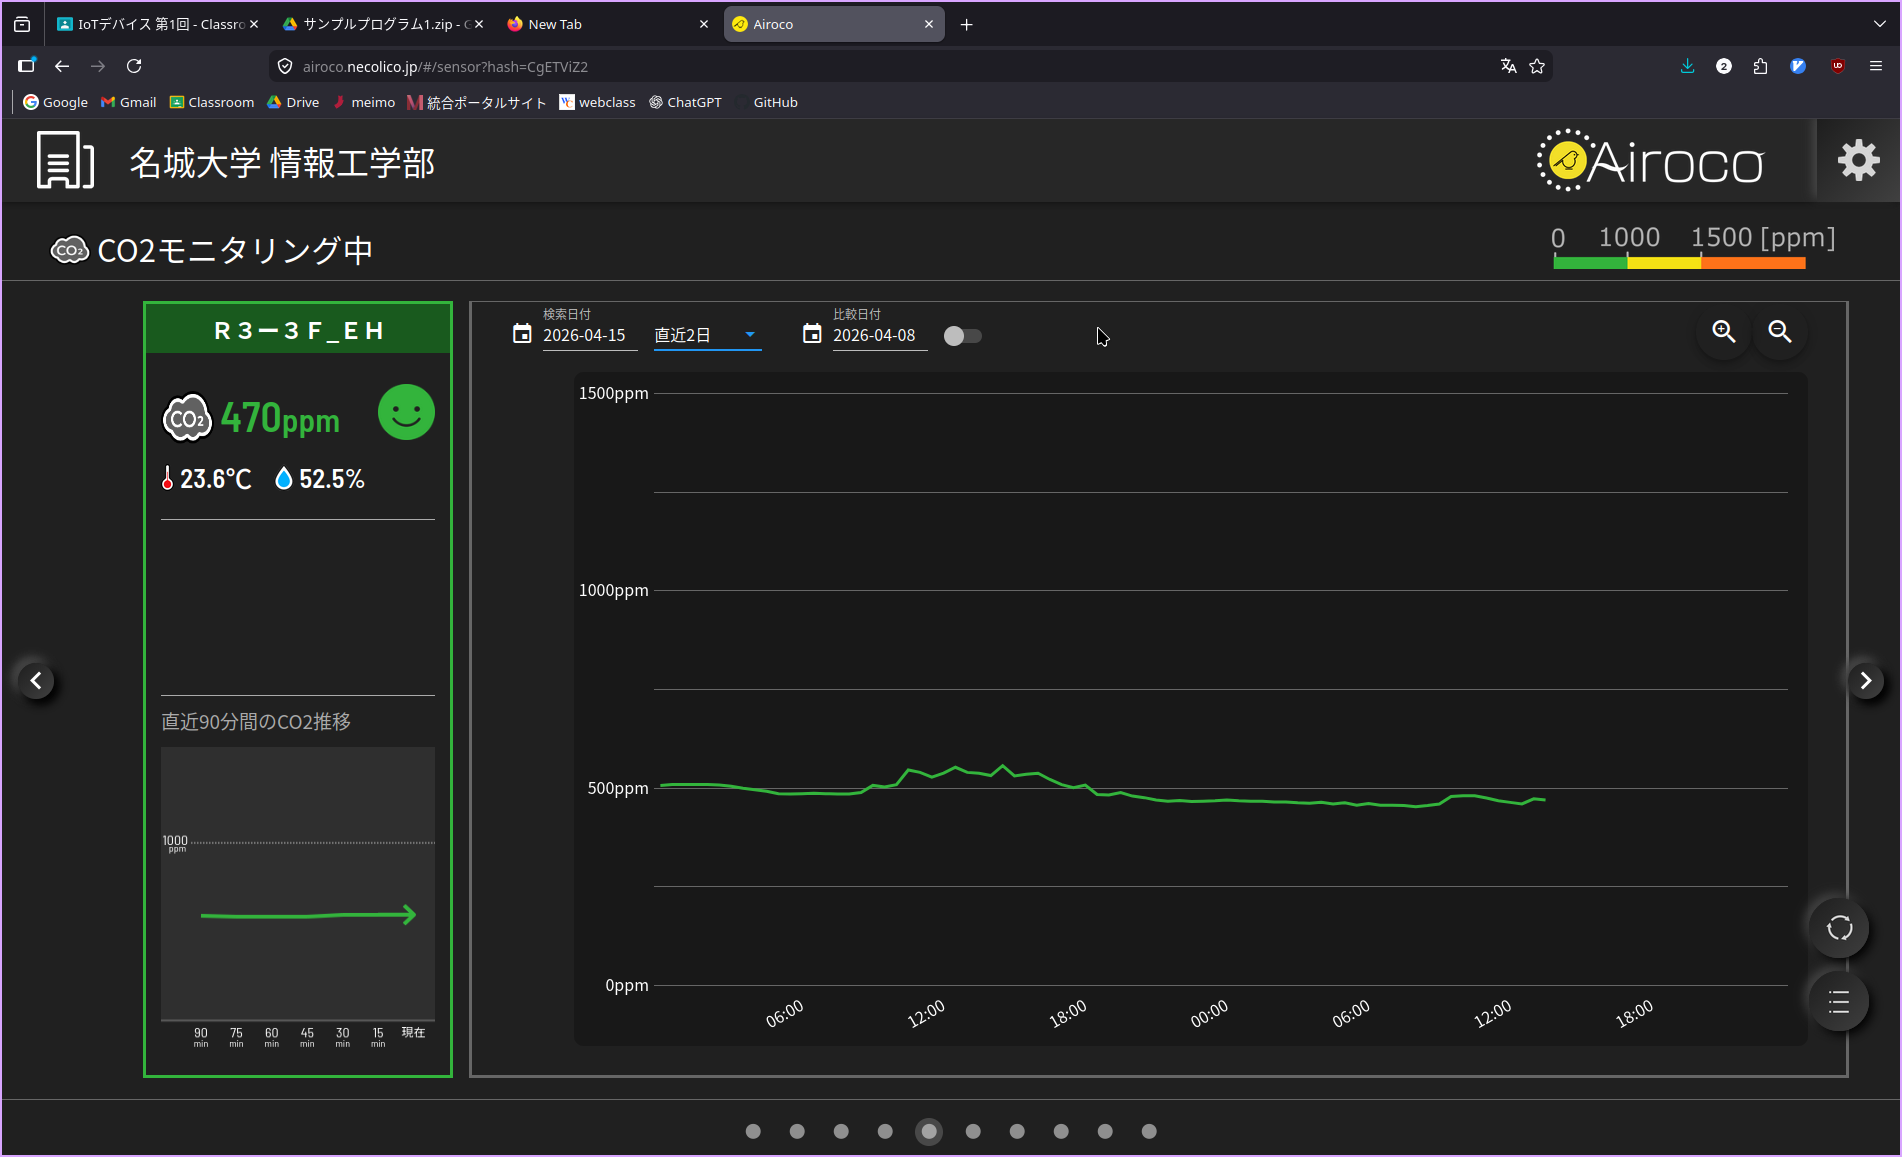
\includegraphics[width=\linewidth]{R3-3F_EH.png}
    \caption{3FエレベーターホールのCO2濃度}\label{fig:3F}
  \end{subfigure}\hfill
  \begin{subfigure}[b]{0.45\columnwidth}
    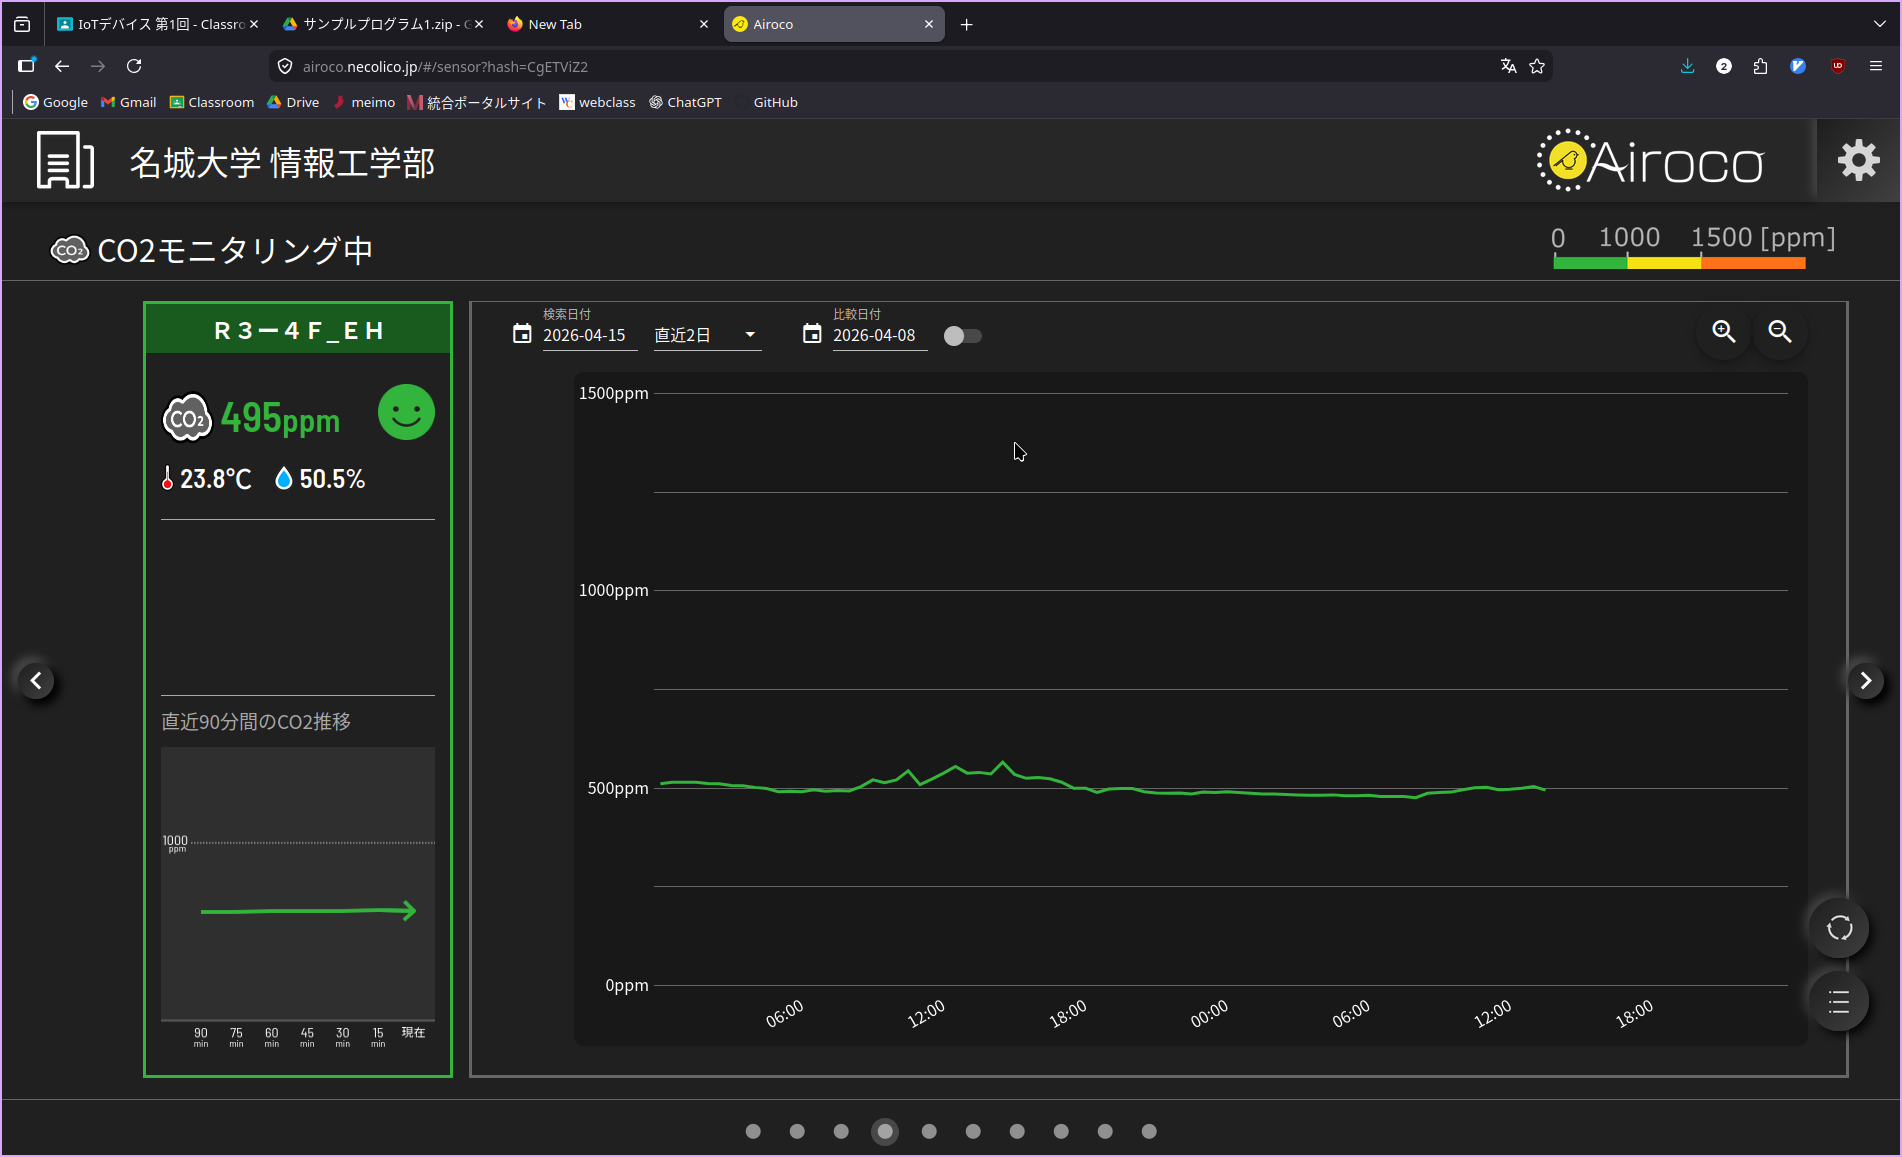
\includegraphics[width=\linewidth]{R3-4F_EH.png}
    \caption{4FエレベーターホールのCO2濃度}\label{fig:4F}
  \end{subfigure}
  \caption{B1Fから4FまでのCO2濃度推移}\label{fig:EH_CO2}
\end{figure}

どのフロアにおいても、9時頃から18時頃にかけてCO2濃度が上昇している。これは、学生・職員等が活動を行っている時間に関係があると考えられる。
また、B1Fに関しては他フロアに比べて格段にCO2濃度が高い。これは、B1Fの学生ラウンジに人が集まりやすいことに関係があると考えられる。特に、昼休み付近の11時から13時にかけて、3限終了ごろから18時にかけてが特に濃度が高いことから、学生がラウンジに集中する時間帯は以下のとおりであると考えられる。


\subsection{1--2}
sample1-2/sample1-2.jsの12行目を見ると、getCsvGraph内でfetch後に  console.log("aaa"); と記述されている。
また、95行目を見ると、getCsvGraph関数を呼び出した後にconsole.log("bbb"); と記述されている。

\begin{figure}[H]
  \centering
  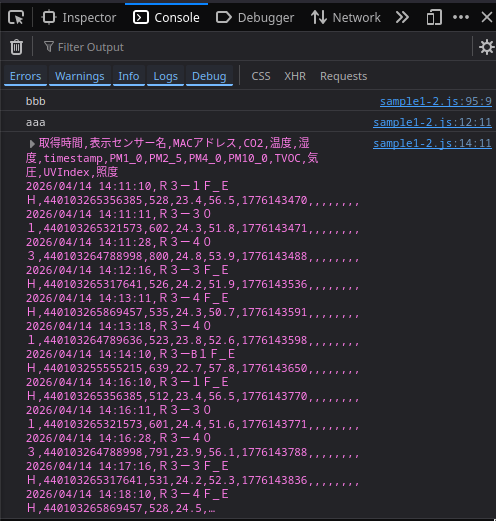
\includegraphics[width=0.5\linewidth]{ex1-2.png}
  \caption{sample1-2.htmlの実行結果}\label{fig:ex1-2}
\end{figure}
実行結果を確認すると、bbb, aaaの順で出力されている。
これは、getCsvGraph関数がasyncつまり非同期処理を行う関数であるため、関数の内部のfetch以前の処理が次の行のconsole.log("bbb");より後に終わったことがわかる。


\subsection{1--3}
pythonを用いてR3-B1F\_EHの過去 1 週間分の CO2 濃度推移をグラフ表示するプログラムを作成した。

作成したグラフを以下に示す。
\begin{figure}[H]
  \centering
  
\includegraphics[width=0.5\linewidth]{ex1-3.png}
  \caption{ex1-3.pyの実行結果}\label{fig:ex1-3}
\end{figure}




%===============================================================================
\end{document}
%===============================================================================

